\section{Methodology}\label{chap:Methodology}
To address the challenges identified in~\cref{chap:Related Work}, namely
evaluation-speed and categorization of near-classes, recent advances in machine
learning are considered. Contrary to most approaches in the field which perform
segmentation, this work focuses on detecting \glspl{bbox}. In this section,
details on the applied method is provided. Methods for object detection can coarsely
be divided into two groups: one-staged and two-staged approaches. To reduce complexity,
only a single one-stage approach will be considered in this paper. For details on
two stage detectors confer e.g.\ \cite{Ren.2015}.

\bigskip
{\large{\textbf{Single Shot MultiBox Detector}}}\\
Two common one-stage architectures are
\gls{yolo}~\cite{Redmon.2015, Redmon.2016b, Redmon.2018} and
\gls{ssd}~\cite{Liu.2016}. While \gls{ssd} can be extended to any base network
(e.g. VGG16~\cite{Simonyan.2015}), \gls{yolo} is limited to only Darknet~\cite{Redmon.2016}.
Therefore, \gls{ssd} was chosen over \gls{yolo} for this paper, retaining the
ability to quickly exchange base networks.

Central concepts of \gls{ssd} are described in the following.

\subsection{Default Boxes}\label{subsect:default-boxes}
The most fundamental part of understanding \gls{ssd} is understanding its specific
concept of \glspl{bbox}, default boxes and anchors. In order to reduce the very high
complexity, this subsection is written in a slightly more colloquial manner.

Slightly anticipating and simplifying \cref{subsect:SSD Architecture}, a
\emph{prediction} from \gls{ssd} is the output from a set of \glspl{convolutional layer}
that is chosen from within the network. Output of a single such \gls{layer} is,
first and foremost, just a \gls{feature map} --- while the goal is to find the
coordinates of a \gls{bbox} (and class predictions). 

Consider such a \gls{feature map} with dimensions \(m \times n\). Every pixel
from that \gls{feature map} contains highly condensed information about a specific
region from the original image\footnote{This concept is called the
\emph{receptive field} of \glspl{cnn}, \cite[cf.][331\psq]{Goodfellow.2016}}.
The \gls{feature map} is then processed further, s.t.\ for every such
pixel (and therefore the related region within the original image) receive the
coordinates of a single \gls{bbox} are received (simplified, for details see \cref{subsect:SSD Architecture}).

To the reader, this might be confusing. Receiving \(m\times n\)
single \gls{bbox} predictions for every pixel within the \gls{feature map} for
every chosen layer makes the number of predicted \glspl{bbox} \(\gg\) than the
expected number of \gls{gt} \glspl{bbox}. And it raises a pressing question:\linebreak
\textbf{How is training data constructed for such an unusual architecture?}

This question is answered (partly) by the introduction of \textbf{anchors}.

\paragraph{Anchors}\label{par:anchors}
Every pixel from a \gls{feature map} is related to a region within the original
input image (\emph{receptive field}~\cite[cf.][331\psq]{Goodfellow.2016}).
Furthermore, \glspl{convolutional layer} preserve the spatial structure of a
convolved image~\cite[cf.][335\psqq]{Goodfellow.2016}.

Therefore, every \emph{pixel} from within the feature map can be related
(very easily) to a region within the original image. The center of such region
is called the \textbf{anchor}. The x and y coordinates for every pixel \(p_{ij}\)
can then be calculated using \cref{eq:anch-x,eq:anch-y}. A practical example for an
image \(I\) of height and width \(I_w\times I_h=300\times 300\) and a
\gls{feature map} \(M\) of height and width \(M_w\times M_h=19\times 19\)
is shown in \cref{fig:vgg16-anchors}.

\begin{align}
    x_i&=0.5*\frac{w_I}{w_M} + \sum_{0}^{i-1} \frac{w_I}{w_M}\label{eq:anch-x}\\
    y_j&=0.5*\frac{h_I}{h_M} + \sum_{0}^{j-1} \frac{h_I}{h_M}\label{eq:anch-y}
\end{align}
where:
\begin{conditions}
    x_i & := & x-coordinates of the anchor for pixel \(p_{ij}\)\\
    y_j & := & y-coordinates of the anchor for pixel \(p_{ij}\)\\
    w_I & := & width of input image \(I\)\\
    w_M & := & width of feature map \(M\)\\
    h_I & := & height of input image \(I\)\\
    h_M & := & height of feature map \(M\)
\end{conditions}
\begin{figure}[t!]
    \centering
    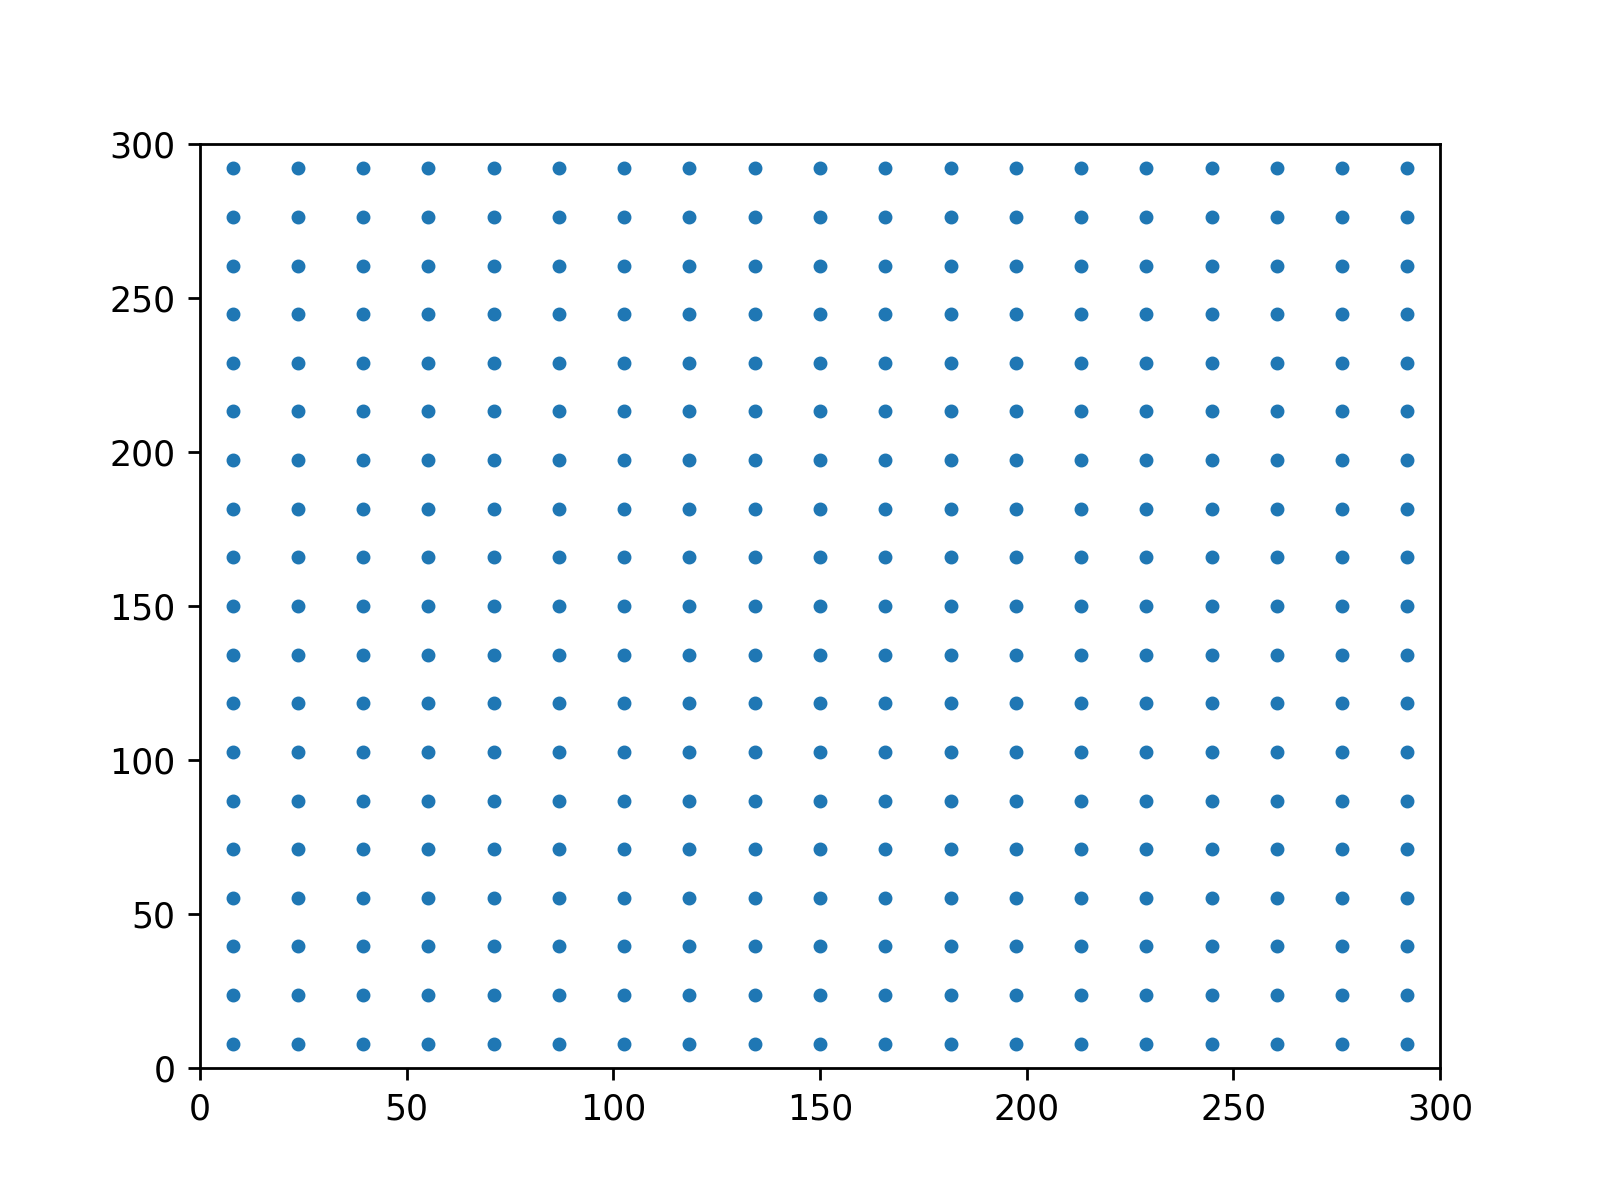
\includegraphics[width=0.5\textwidth]{vgg16-19x19}
    \caption{Generated anchors (blue) for an image of dimensions \(300\times 300\)
    and \gls{feature map} of \(19\times 19\).}\label{fig:vgg16-anchors}
\end{figure}
Now, training data could be constructed by assigning every \gls{gt} \gls{bbox} to
its closest anchor (from every chosen layer). An example of this is given in
\cref{eq:train-anchor}. 
\begin{equation}\label{eq:train-anchor}
    \begin{matrix}
        \ldots\\
        \begin{bmatrix}
            \ldots & \ldots & \ldots & \ldots & \ldots\\
            0 & 0 & 0 & 0 & 0\\
            271 & 828 & 182 & 845 & 1\\
            0 & 0 & 0 & 0 & 0\\
            \ldots & \ldots & \ldots & \ldots & \ldots
        \end{bmatrix}\\
        \ldots\\
        \begin{bmatrix}
            \ldots & \ldots & \ldots & \ldots & \ldots\\
            0 & 0 & 0 & 0 & 0\\
            3141 & 592 & 653 & 59 & 1\\
            0 & 0 & 0 & 0 & 0\\
            \ldots & \ldots & \ldots & \ldots & \ldots
        \end{bmatrix}\\
        \ldots
    \end{matrix}
\end{equation}
where the first four rows are x- and y-coordinate, height and width of the respective
\gls{bbox} and the last row is the class (0: \textit{no-object}, 1: \textit{object}).

This approach is flawed in two ways:
\begin{enumerate}
    \item Assigning \gls{gt} \glspl{bbox} to the closest anchor is entirely agnostic
    of the expected size of the receptive field for the different layers. A layer
    with smaller receptive field per pixel would probably not be able to perceive
    larger objects, while a layer with a larger receptive field might overlook
    smaller objects.\label{itm:anchor-flaw1}
    \item The model has no \textit{a priori} knowledge of \emph{position}, of
    \emph{x-} and \emph{y-coordinates}, of \emph{width} and \emph{height}.
    This is especially critical for images with different resolutions.\label{itm:anchor-flaw2}
\end{enumerate}
A possible solution to these flaws are \textbf{default boxes}.

\paragraph{Default Boxes}\label{par:default-boxes}
Default boxes are used to assign spatial representation to anchors. With such a
representation, every \gls{gt} \gls{bbox} can be matched to the set of regions
(related to the receptive fields) that have a large overlap\footnote{The overlap
could then be computed via \gls{iou} for example --- as is done in \cref{eq:bbox-matcher}.}.

As a starting point, so far a set of chosen layers \(L = \left\{l_0, l_1, \ldots, l_{n-1}\right\}\)
and a set of anchors for every such layer \(\mathbf{A} = \left\{A_0, A_1, \ldots, A_{n-1}\right\}\)
were constructed.

Now, although the exact receptive fields of the chosen layers are uncertain, 
we \emph{do} know that their sizes \(\abs*{recept\left(l\right)}\), are strictly
increasing with subsequent layers, i.e.\ \(\abs*{recept\left(l_0\right)} < \ldots < \abs*{recept\left(l_{n-1}\right)}\).

Fortunately, \textcite{Liu.2016} claim that the exact size of the receptive field is of
subordinate importance. Instead of calculating the exact receptive field, they
propose to assign a fixed size to every chosen \gls{layer} per \cref{eq:default-box-size}:
\begin{equation}\label{eq:default-box-size}
    s_k=s_{_\text{min}} + k * \frac{s_{_\text{max}}-s_{_\text{min}}}{n-1}
\end{equation}
Where
\begin{conditions}
    n               &:= & \(\abs*{L}\)\\
    k               &\in & [0, n-1]\\
    s_{_\text{min}} &=& 0.2\\
    s_{_\text{max}} &=& 0.9
\end{conditions}
A default box \(d_{i,j}\) for a pixel \(p_{i,j}\) within a given layer \(l_k\)
can then be computed as given in \cref{eq:dbox}.
\begin{align}
    \begin{split}\label{eq:dbox}
        d_{i,j}^h  &= s_k * h_I\\
        d_{i, j}^w &= s_k * w_I\\
        d_{i,j}^x  &= x_i \text{ (see \cref{eq:anch-x})}\\
        d_{i,j}^y  &= y_j \text{ (see \cref{eq:anch-y})}
    \end{split}
\end{align}
It is now possible to match every \gls{gt} \gls{bbox} to a set of default boxes
(see \cref{eq:bbox-matcher}).
\begin{equation}\label{eq:bbox-matcher}
    match(\text{bbox}, \text{dbox}) =
    \begin{cases}
        1 & \text{if } \text{IoU}\left(\text{bbox, dbox}\right) > 0.5\\
        0 & \text{otherwise}
    \end{cases}
\end{equation}
where:
\begin{conditions}
    \text{bbox} & := & coordinates of the bounding box\\
    \text{dbox} & := & coordinates of the default box
\end{conditions}
Thereby, \hyperref[itm:anchor-flaw1]{\(\left.\text{flaw 1}.\right)\)} from anchor
construction can be considered as solved.

\hyperref[itm:anchor-flaw2]{\(\left.\text{Flaw 2}.\right)\)} can now be tackled
multiple ways. The most obvious would be to convert \gls{gt} \glspl{bbox} and
default boxes into the \textit{percental} space (i.e. \(\left[0, 1\right]\)).
Yet, this again would require the model to learn different semantics per pixel
within a \gls{feature map}. For example, the upper left pixel/region would produce predictions
within \(\left[0,0.2\right]\times \left[0,0.2\right]\), while the lower right
region would produce predictions within \(\left[0.8,1.0\right]\times \left[0.8,1.0\right]\).
This is problematic, because \glspl{convolutional layer} share weights\footnotemark{}
between inputs (i.e. such pixels/regions)~\cite[cf.][564\psqq]{Murphy.2012}.
\footnotetext{In fact, sharing weights between inputs is the key distinguishing
feature between \glspl{convolutional layer} and \glspl{dense layer}.}
Requiring different semantics \emph{between} these pixels introduces additional
complexity to the \glspl{convolutional layer}.

To alleviate this complexity, rather than coordinates, the offset \emph{between}
the coordinates (of \gls{gt} \glspl{bbox} and the related default boxes) are predicted.
This aligns the task between all pixels of a \gls{feature map}.

\Textcite{Liu.2016} introduce a last quirk inspired by the concept of priors
from bayesian statistics~\cite[cf.][165\psqq]{Murphy.2012}. To improve convergence
they choose multiple aspect ratios (i.e.\ 1:1, 1:2, 1:3, 2:1, 3:1) for their
default boxes. Reducing extent of this paper, the reader is referred to \cite{Liu.2016}.

Finally, the sets of default boxes per \gls{layer} are concatenated and further
encoded as described in \cref{append:Concepts of Bounding Box Encoding}, such
that default box

Digressing slightly, a common method in statistics (especially bayesian~\cite[cf.][165\psqq]{Murphy.2012})
is the usage of \textbf{priors} as a means to express \textit{a priori} beliefs about a task.
Such a prior is then (given that the expressed belief holds) able to help improve
model fit\footnotemark. In \gls{ssd},
default boxes are a prior that is expressing \textit{a priori} information about
the dimensions of cars, pets, pedestrians, objects from the real world in general
(or whatever else is found within training data).

\footnotetext{Note that this is a simplification. The concept of priors is
a central part of bayesian statistics and not merely a way to improving model
fit. Please consider \cite[165\psqq]{Murphy.2012} for details.}

To ease this challenge of finding the coordinates of such a \gls{bbox} a
\textbf{prior} is deployed. \textbf{This} is the purpose of \textbf{default boxes}
and \textbf{anchors}.

\subsection{Encoding Ground Truth} For training, ground truth \glspl{bbox}
are encoded with respect to the concatenated default boxes as calculated in
\cref{par:default-boxes}. 


\gls{ssd} is supposed to infer offsets to default
boxes (cf. \cref{subsect:SSD Architecture}). To simplify inference only default
boxes with an \gls{iou} greater than 0.5 are chosen (cf. \cref{sect:Intersect Over Union}). For a \gls{bbox}
\(\text{bbox}=\{\text{bbox}_{x_\text{min}}, \text{bbox}_{x_\text{max}}, \text{bbox}_{y_\text{min}}, \text{bbox}_{y_\text{max}}\}\), default box
\(\text{dbox}=\{\text{dbox}_{x_\text{min}}, \text{dbox}_{x_\text{max}}, \text{dbox}_{y_\text{min}}, \text{dbox}_{y_\text{max}}\}\) we compute the
encoded box \(\text{ebox}\) with \cref{eq:encoded box}
\begin{equation}
    \text{ebox}=\{(\text{bbox}_{x_\text{min}}-\text{dbox}_{x_\text{min}}), (\text{bbox}_{x_\text{min}}-\text{dbox}_{x_\text{max}}), (\text{bbox}_{y_\text{min}}-\text{dbox}_{y_\text{max}})\}\label{eq:encoded box}
\end{equation}
We receive a matrix of dimensions \(\sum_{m\in M}{A_m}\times \sum_{m\in M}{k_m*4}\),
where \(M\) is the set fo all \glspl{feature map}, \(A_m\) is the set of all anchors per
\gls{feature map} and \(k_m\) is the amount of aspect ratios per \gls{feature map}. Finally
we concatenate the class label to every encoded \gls{bbox}, such that the matrix
dimensions now are \(\sum_{m\in M}{A_m}\times \sum_{m\in M}{k_m*4+c}\), where c
is the amount of classes. Every row is now in the form of
\begin{equation}
    \left\{x_{_\text{min}}, x_{_\text{max}}, y_{_\text{min}}, y_{_\text{max}}, \text{one\_hot\_classes} \right\}
\end{equation}


\subsection{SSD Architecture}\label{subsect:SSD Architecture}
As mentioned in the introduction to this section, \gls{ssd} is independent of any
specific base network. Exemplary, \cref{fig:ssd-vgg} shows the architecure of
SSD for VGG16~\cite{Simonyan.2015}. Fully connected \glspl{layer} of VGG16 are
dropped and replaced with additional \glspl{convolutional layer}. We denote: 
\(\text{Network}:=\text{Base Network}\rightarrow \text{Additional Layers}\).

Then, a set of \glspl{convolutional layer} \(L\) (blue and yellow in \cref{fig:ssd-vgg})
is chosen from the network (i.e.\ \(L\subseteq \text{Network}\))\footnote{\label{foot:receptive}The motivation
behind choosing multiple layers \(L\) from the network is as follows: the \glspl{feature map}
produced by the \glspl{convolutional layer} get smaller with every additional layer.
Colloquially speaking, the relationship between such a small \gls{feature map} and
the input image is, that one pixel within the small \gls{feature map} is related
to multiple pixels within the original input image. Therefore, when looking at the
\glspl{feature map} from subsequent \glspl{convolutional layer}, one is looking
at information that is extracted from the image at different scales.

Making this logic concrete, in a larger \gls{feature map}, one pixel might contain
condensed information about objects like wheels or headlights, whereas in a smaller
\gls{feature map} one pixel might contain  condensed information about the entire
car. This concept is called the \textit{receptive field}~\cite[cf.][331\psq]{Goodfellow.2016}.}.

To produce class- and \gls{bbox} predictions, every chosen \glspl{layer} \(l\in L\)
is directed into a final additional \gls{convolutional layer} (i.e.\ one additional
\gls{convolutional layer} per \gls{layer} in \(L\), depicted green in \cref{fig:ssd-vgg}).

Das hier setzt halt alles Wissen voraus, das noch gar nicht aufgebaut wurde!

The number of filters for these subsequent \glspl{layer} is chosen as \((4+c)*k\)
with \(c\) classes\footnote{Actually, \(c+1\) classes. This additional class is
the \textit{no-class}-prediction, because obviously most areas within the image
contain no classifiable object.} and \(k\) default boxes per \gls{anchor}.
\begin{figure}[ht]
    \centering
    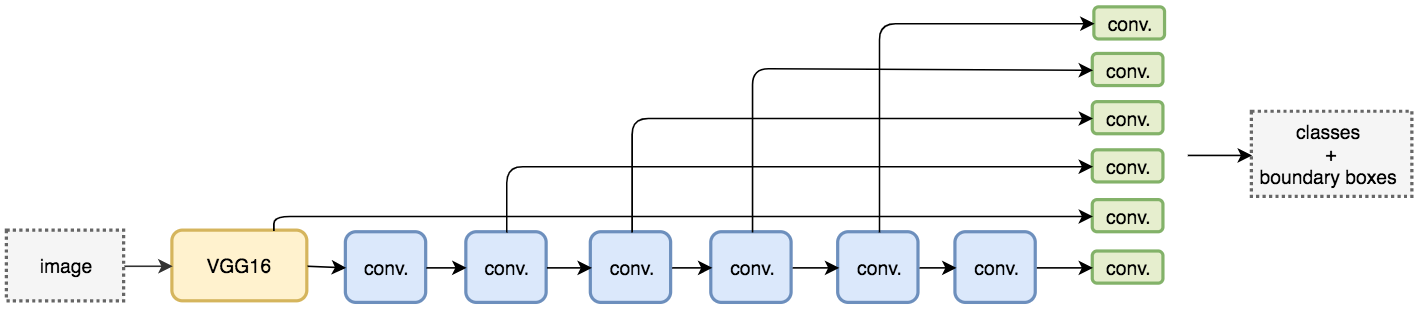
\includegraphics[width=1\textwidth]{vgg16-ssd}
    \caption[Example of the SSD architecture using VGG16 as its base network]{Example
    of the SSD architecture using VGG16 as its base network~\cite[cf.][]{Liu.2016}.
    \\\\
    Blue colored boxes represent the additional \glspl{convolutional layer} that are added to the base network.
    \\\\
    Green boxes represent the final additional \glspl{convolutional layer} that produce
    the classes- and \gls{bbox} predictions.}
    \label{fig:ssd-vgg}
\end{figure}

\subsection{Training}
\ldots

\subsubsection{Loss Function}
The loss is a composite of two separate loss functions:

\begin{align}
    L_{\text{conf}(x, c)}\\
    L_{\text{loc}(x, l, g)}\\
    L(x,c,l,g) = \frac{1}{N}*\left(L_{\text{conf}(x, c)} + \alpha * L_{\text{loc}(x, l, g)}\right)
\end{align}

\begin{equation}
    \begin{cases}
        L(x,c,l,g) = \frac{1}{N}*\left(L_{\text{conf}(x, c)} + \alpha * L_{\text{loc}(x, l, g)}\right),& \text{if } N \geq 1\\
        0, & \text{otherwise}
    \end{cases}
\end{equation}

\begin{equation}
    L_{\text{loc}(x, l, g)} = \sum_{i \in Pos }^{N}
\end{equation}
where:
\begin{conditions}
    N & := & number of matched boxes\\
    x & := & pixel under consideration\\
    c & := & class scores\\
    l & := & Predicted Boxes\\
    g & := & Ground Truth Boxes\\
    \alpha & := & weighting parameter, increase to put importance on the localization loss.
\end{conditions}
